\section{Software}

\subsection{Generel struktur}

\subsection{Kommunikations Protokol}
I oplægget er der specificeret en kommunikationsprotokol som bilen skal overholde. Protokollen fungerer ved hjælp af telegrammer. I afsnittet "Beskrivelse af telegram" forklares der, hvad et telegram er. Og i afsnittet "Implementering" beskrives der, hvordan protokollen kodemæssigt er implementeret i microcontrolleren.\\
Al kode der omhandler kommunikations protokollen ligger i .asm-filen "Communication\_Protocol.asm"

\subsubsection{Beskrivelse af telegram}
Protokollen er baseret på "telegrammer" bestående af 3 bytes der henholdsvis repræsenterer en type, kommando og et parameter.\\
Af typer er der specificeret 3 forskellige:
\begin{itemize}
	\item SET - 0x55 - Bruges til at sætte en værdi i bilen
	\item GET - 0xAA - Bruges til at hente en værdi fra bilen
	\item REPLY - 0xBB - Bruges til når der returneres en værdi som svar på et get/set telegram
\end{itemize}
Det har ikke været nødvendigt at implementerer yderligere typer, så dette er også de eneste tre typer som implementeringen gør brug af.\\
Af kommandoer er der fra oplæggets side sat et krav om to som bilen som minimum skal overholde, disse er som følger:
\begin{itemize}
	\item Start - 0x10 - Bruges til at starte bilen med en procentdel af maxspændingen ud 			fra parametret
	\item Stop - 0x11 - Bruges til at stoppe bilen med
\end{itemize}

Ud over dette har vi specificeret yderligerer to set kommandoer:
\begin{itemize}
	\item Speed\_H - 0x12 - Bruges til at sætte de øverste 8 bit af en 16-bit værdi der essentielt bestemmer hvilken hastighed hastighedskontrollen forsøger at holde
	\item Speed\_L - 0x13 - Bruges til at sætte de nederste 8 bit af en 16-bit værdi der essentielt bestemmer hvilken hastighed hastighedskontrollen forsøger at holde
\end{itemize}

Disse to kommandoer er essentielt en kommando, men skal sendes som to seperate kommandoer da et telegram kun kan bestå af en type, kommando og et parameter. De er blevet brugt meget til at teste hastighedskontrollen af og fastsætte max hastigheder rundt i forskellige sving.\\

Fra oplæggets side er der ikke specificeret nogle get kommandoer, men vi har implementeret de følgende:
\begin{itemize}
	\item Xaccel\_H - 0xA1 - Returner de øverste 8 bit af den signerede 16-bit rå værdi fra acceleration af x-aksen på sensoren
	\item Xaccel\_L - 0xA2 - Returner de nederste 8 bit af den signerede 16-bit rå værdi fra acceleration af x-aksen på sensoren
	\item Zgyro\_H - 0xA3 - Returner de øverste 8 bit af den signerede 16-bit rå værdi af vinkelhastigheden om z-aksen på sensoren
	\item Zgyro\_L - 0xA4 - Returner de nederste 8 bit af den signerede 16-bit rå værdi af vinkelhastigheden om z-aksen på sensoren
	\item Ticks\_H - 0xA5 - Returner de øverste 8 bit af den 16-bit værdi der fortæller, hvor mange "ticks" bilen har kørt på daværende tidspunkt
	\item Ticks\_L - 0xA6 - Returner de nederste 8 bit af den 16-bit værdi der fortæller, hvor mange "ticks" bilen har kørt på daværende tidspunkt
	\item LapTime\_H - 0xA7 - Returner de øverste 8 bit af den 16-bit værdi der fortæller, hvor mange millisekunder banen tog at gennemfører
	\item LapTime\_L - 0xA8 - Returner de nederste 8 bit af den 16-bit værdi der fortæller, hvor mange millisekunder banen tog at gennemfører
	\item LapTicks\_H - 0xA9 - Returner de nederste 8 bit af den 16-bit værdi der fortæller, hvor mange "ticks" der har været på en omgang af banen
	\item LapTicks\_L - 0xAA - Returner de nederste 8 bit af den 16-bit værdi der fortæller, hvor mange "ticks" der har været på en omgang af banen
	\item Data - 0xAB - Bliver brugt til at få bilen til at returnerer flere data-værdier uden at skulle sende et get telegram for hver enkelt. Justeres ind alt efter hvad man gerne vil have tilbage.
	
\end{itemize}

Til sidst i telegrammet sendes der altid et parameter med, også selvom en funktion ikke gør brug af et parameter.

\subsubsection{Implementering}
Implementeringen kan deles op i to dele, en del der står for at behandle de modtagne bytes. Og en del der står for at eksekverer kommandoerne når et helt telegram er modtaget. 

\paragraph{Modtagelse}
\textit{Figur \ref{fig:Comm_Modtagelse} Beskriver modtagelsen som et flowchart.} \\

Når USART modulet modtager en byte vil der blive kaldt et interrupt der springer til plads 0x1A, hvor kommandoen "jmp Comm\_Received" står. Dette er indgangen til modtagelsesdelen af implementeringen. \\
Først indlæses værdien Byte\_Num fra SRAM. Den holder styr på, hvilken af de 3 bytes der er modtaget. Den første byte, altså typen, har værdien et. Ud fra denne værdi springer programmet så til håndteringen af en modtaget type, modtaget kommando eller en eksekvering af det modtagende telegram. Håndteringen af typer og kommandoer er den sammen. Den modtagende type/kommando holdes op mod de typer/kommandoer som microcontrolleren kender og hvis det er en kendt type/kommando så gemmes den i SRAM og Byte\_Num inkremeres med en. Hvis det derimod ikke er en kendt type/kommando så sættes Byte\_Numb til en og derved smides telegrammet væk, hvis ikke det er af en type som der er implementeret i microcontrolleren. Den første implementering af kommunikations protokollen indeholdt ikke dette check for om det var en godkendt type allerede i modtagelsen. Dette gjorde at hvis der på en eller anden måde fik sneget sig en byte ind imellem modtagelsen af type, kommando og parameter. Så ville microcontrolleren skulle modtage 3 bytes før fejlen bliver opdaget. Dette resulterede i at efterfølgende telegrammer ville være forskubbet med en byte og konsekvent ville fejle. Med den nuværende implementering vil microcontrolleren opdage fejlen med det samme og efterfølgende telegrammer vil blive opfanget korrekt. Grunden til reimplementeringen var at når man sendte telegrammer hurtigere end microcontrolleren kunne håndterer dem så begyndte dens rx-buffer at blive overskrevet og dette fik meget hurtigt ødelagt kommunikationen pga. forskubbede telegrammer. Den nuværende implementering lider ikke under dette og vil blot ikke svarer på en kommando ,hvis den oplever et overflow, men svarer efterfølgende igen når dens buffer ikke oplever et overflow længere. Dette gør protokollen meget mere solid.

\begin{figure}[p]

	\centering
		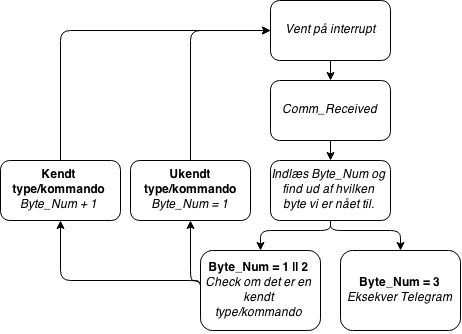
\includegraphics[scale=0.8]{Billeder/Comm_Modtagelse.png}
	\caption{Flowchart over kommunikations protokollen ved modtagelsen af en byte)}
	\label{fig:Comm_Modtagelse}
	
\end{figure}

\paragraph{Eksekvering} 
\textit{Figur \ref{fig:Comm_Eksekvering} Beskriver eksekveringen som et flowchart.} \\
Eksekveringen bliver kørt når byte nummer 3, parametret, bliver modtaget. Her bliver typen og kommandoen igen tjekket for at finde ud af, hvilken kommando der skal eksekveres. Hvis der af en eller anden grund er en fejl på de SRAM addresser der indeholder typen og kommandoen. Så vil microcontrolleren ikke genkende det gemte telegram og selv resette igen. Så kommunikationen kan fortsætte bagefter uden at den hænger eller forskyder telegrammerne. Efter eksekveringen af kommandoen er endt så vil Byte\_Num blive sat til en igen og det hele vil begynde forfra.

\begin{figure}[p]

	\centering
		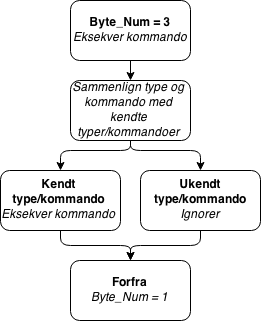
\includegraphics[scale=0.8]{Billeder/Comm_Eksekvering.png}
	\caption{Flowchart over kommunikations protokollen ved eksekveringen af en byte)}
	\label{fig:Comm_Eksekvering}
	
\end{figure}

\subsection{Eksempler(sensor)}

\subsubsection{Tachometer}

Til at behandle signalet fra hall sensoren, benyttes input capture funktionen til Timer 1. Input capture funktionen har sit eget interrupt og fungerer ved automatisk at læse værdien af Timer 1's timer/counter registre (TCNT1A/TCNT1B) over i to input capture registre (ICR1L/ICR1H) når der kommer et interrupt. Input capture er den sekundære funktion til PD6, og sættes op i Timer 1's kontrol registre (TCCR1A/TCCR1B). Vi valgte at sætte den op med en prescaler på 1/8 og en falling edge interrupt trigger. Det giver en opdateringsfrekvens på 0.5 $\mu s$ og en maksimal tid på 32.5 ms inden timer/counter registrene overflower. Det er fint nok til at kunne rumme tiden imellem flere interrupts. I interruptrutinen beregnes tiden imellem 4 interrupts for at finde ud af hvor lang tid motoren er om at dreje en omgang (Der sidder tre poler på motoren, så 4 interrupts vil svare til en hel omgang for motoren). Denne tid kan så bruges som et udtryk for hastigheden, da de to ting er omvendt proportionale. Bilens reelle hastighed kan også beregnes, men på grund af proportionaliteten er det ligegyldigt, fra microcontrolleren's synspunkt, om man bruger det ene eller det andet - man skal bare huske at en høj hastighed vil give en lav tid og omvendt, når man skriver programmet, der skal bearbejde hastigheden. Jo færre cycles man bruger på at få noget brugbart ud i den anden ende jo bedre, i næsten alle tilfælde, når der også skal laves andre ting sideløbende med input capture interruptet.\\
For at beregne tiden skal der holdes styr på pulserne - der skal bruges en tid fra den første puls og en tid fra den sidste puls. Det letteste er at tælle en variabel op, hver gang der modtages et interrupt således at, når variablen er 1 så læser man den første tid, og når variablen er 4 så læses den sidste tid. Derefter trækkes de to tider fra hinanden for at finde forskellen. Alle værdier og variable gemmes i SRAM-hukommelsen på tildelte addresser indtil de skal bruges igen.\\

Det viste sig at hall sensoren gav mange udslag når bilen holdt stille og en af polerne var lige på grænsen til at passere sensoren. Vi antager at det er fordi feltet er meget ustabilt i grænseområdet. 


\subsubsection{Lap sensor}

For at initialisere microcontrolleren's komparator skal den sættes op i dens eget status register (ACSR) og i Special Function IO Registret (SFIOR). Man kan vælge flere forskellige inputs til komparatoren - PB2(AIN1) og PB3(AIN0) er henholdsvis ikke-inverterende og inverterende inputs som standard. Alternativt kan hele PORTA bruges til det inverterende og den interne bandgap reference på 2.56 V til det ikke-inverterende.  ACME bit'en i SFIOR enabler ADC multiplexeren, så den styrer hvilket ben på PORTA der bliver brugt. ACBG bit'en enabler bandgap referencen.

\begin{figure}[h]

	\centering
		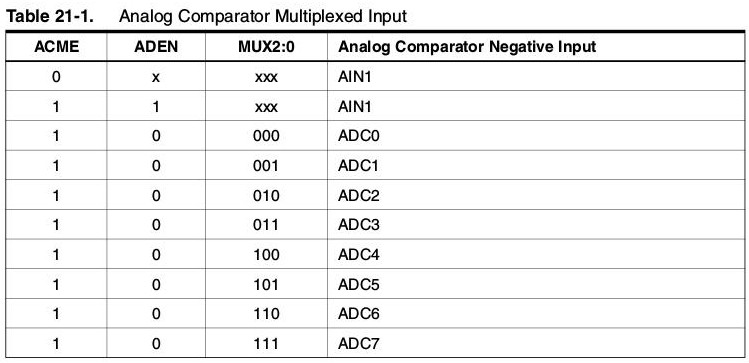
\includegraphics[scale=0.3]{Billeder/Table21-1.jpg}
	\caption{I tabellen kan man se at ACME bit'en lader multiplexeren vælge hvilket ben på PORTA, der er input til komparatorens inverterende ben. Medmindre ADC'en er slået til - så bliver inputtet taget fra PB2(AIN1)}
	\label{fig:ACME}
	
\end{figure}

Man har også mulighed for at vælge, hvornår komparatoren skal sende et interrupt. Interruptet bliver sendt som en reaktion på hvad der sker på komparatorens output-ben. Vi har sat den op til at sende et interrupt, når outputtet toggler tilstand, men der er også mulighed for at køre på enten falling eller rising edge. Det betyder i vores tilfælde ikke noget hvilken metode man vælger på grund af måden koden bearbejder interruptet, men mere om det senere.\\

I interruptrutinen til lap sensoren beregnes omgangstiden. Hver gang målstregen krydses læses tiden fra tre SRAM addresser, hvor tiden microcontrolleren har været tændt millisekunder er gemt i 24 bits. Interruptrutinen sørger for at gemme et 24 bits time stamp i SRAM'en hver gang den køres. Med den totale tid og et time stamp fra det forrige interrupt, er det bare et spørgsmål om at trække de to fra hinanden for at finde omgangstiden. For at forhindre ugyldige omgangstider, hvis der kommer mere end et interrupt på samme målstreg, kontrolleres det om omgangstiden er længere end 512 millisekunder se figur \ref{fig:LapTime}.

\begin{figure}[h]

	\centering
		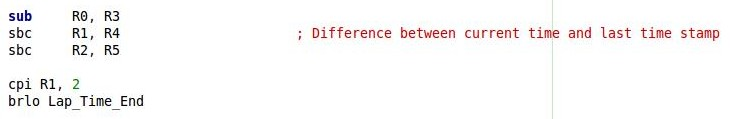
\includegraphics[scale=0.5]{Billeder/LapTime.jpg}
	\caption{Her er den nuværende tid gemt i R0, R1, R2 og time stampet i R3, R4, R5. Ved at kontrollere om den mellemste byte i R1 er under 2 kan det afgøres, om der er gået nok tid siden sidste time stamp til at anse interruptet som gyldigt.}
	\label{fig:LapTime}
	
\end{figure}

Det er også efter denne kontrol at man kan ændre på alle de parametre der kun skal ændres en gang når målstregen krydses. Inden man forlader interruptrutinen er det vigtigt at resette comparator interrupt flaget i ACSR. Hvis flaget er sat, når det globale interrupt bliver enablet efter rutinen, anser microcontrolleren det som om den har modtaget et nyt interrupt, og så vil den køre hele rutinen igen.

\subsection{Hastighedskontrol}

For at designe en hastighedskontrol, der selv regulerer PWM og bremser alt efter hvor langt den målte hastighed er fra den ønskede, valgte vi at designe en progressiv kontrol, hvorved jo større forskellen imellem den ønskede og målte hastighed er, jo kraftigere vil microcontrolleren forsøge at justere. Tanken er at bruge den forskel som et direkte input til OCR2 eller bremsen, således at jo tættere bilen kommer på den ønskede hastighed jo lavere bliver værdien i OCR2, og lige sådan omvendt. Det medfører at det er umuligt for bilen at stabilisere sig selv på den ønskede hastighed, men det gør ikke det store, da den ønskede hastighed er i forvejen en arbitrær værdi, som man skal eksperimentere sig lidt frem til. Det er både fordi det ikke kan vides på forhånd, hvilke hastigheder der er ideelle i alle situationer, men også fordi den værdi microcontrolleren justerer efter ikke er en rigtig hastighed men tiden pr. motoromdrejning.\\
Hastighedskontrollen er implementeret som en call-funktion, der bliver kaldt hver gang hastigheden bliver opdateret i input capture interruptrutinen. Det har den ulempe, at hvis bilen går i stå, af en eller anden grund, så der ikke kommer flere interrupts, så kan den ikke starte igen af sig selv, hvis værdien i OCR2 er 0. \\
\paragraph{PWM}
 Det første der sker er at den ønskede og den målte hastighed læses ind fra SRAM'en og derefter findes forskellen mellem dem. For at afgøre om bilen kører for hurtigt eller for langsomt, kontrolleres fortegnet på den udregnede forskel - det kan gøres nemt ved at kigge på N-flaget i statusregistret. Hvis bilen kører for langsomt er forskellen negativ og for at kunne arbejde med det bruges tallets to-komplement. Hvis forskellen er større end en på forhånd bestemt størrelse så sættes OCR2 til 255 så duty cycle er på 100 procent. Hvis den er under læses forskellen direkte ind i OCR2. Eller det ville vi gøre, hvis hastigheden var en 8-bits værdi - vi gemmer hastigheden som en 16 bits størrelse så derfor er vi nødt til at dividere tallet ned så det passer i et 8 bits register. Så længe man bibeholder proportionaliteten gør det ikke noget at tallet bliver divideret ned. For at spare på cycles i en interruptrutine, der bliver kaldt forholdsvis ofte, divideres der kun med potenser af 2 - det kan laves nemmere ved at bruge logic shifts eller rotations (det svarer til at flytte kommaet, når man ganger eller dividerer med 10 i base-10 talsystemer). Ved at dividere tallet ned giver det også muligheden for nemt at sætte et maksimum på værdien, der kan læses ind i OCR2, når forskellen bliver brugt direkte. Hvis man eksempelvis sætter max-forskellen til 5760 så kan der højest læses 180 ind i OCR2, inden microcontrolleren regulerer med fuld kraft, idet $180 \cdot 32 = 5760$. Jo større tal man dividerer med, jo blødere reguleres motorkraften og jo større skal forskellen også være, for at der gives fuld kraft på motoren - vi fandt en udemærket balance på 32.\\

\paragraph{Bremse}
Bremsen fungerer efter samme princip, men den regulerer bare bremsen med en tid i millisekunder. Når forskellen bliver positiv læses der som standard 0 ind i OCR2 så duty cycle også bliver 0 - der sættes også en bit på en SRAM-addresse, som fortæller at bilen er igang med at bremse. Helt i starten af hastighedskontrollen checkes denne bit og hvis den er sat, springer program counteren til en anden funktion, der holder øje med hvor lang tid der har været bremset i. Funktionen fungerer meget på samme måde som den der holder øje med omgangstider - der sættes et time stamp lige når bremsen bliver sat til, og så holder microcontrolleren øje med om der forløbet nok tid til at den kan slå bremsen fra igen. Tiden bremsen er sat til i, bliver på samme måde som med PWM, når bilen kører for langsomt, ved at bruge hastighedsforskellen som direkte parameter. Den maksimale tid der bremses i med er 255 ms - det viste sig under tests at en bremsetid på mere end 255 ms ikke har ret meget effekt. Samtidig kan man genbruge 8 bits formatet fra tidligere. Bilen finder selv ud af om der er brug for at bremse mere efter de 255 ms er gået. Der er indbygget en lille buffer, så bremsen ikke bliver brugt lige så snart forskellen bliver positiv - op til en vis grænse er der en slags soft braking zone se figur \ref{fig:Forgiveness}, hvor OCR2 bare er sat til 0. 

\begin{figure}[h]

	\centering
		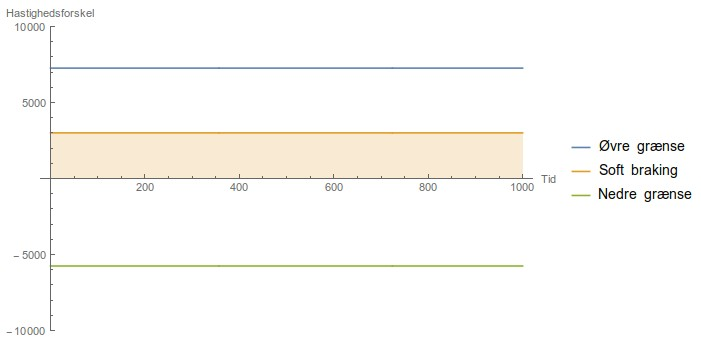
\includegraphics[scale=0.5]{Billeder/Braking.jpg}
	\caption{Ned til den nedre grænse bruge forskellen direkte i OCR2. I soft braking zonen læses 0 ind i OCR2 - derfra og op til den øvre grænse bruges bremsen i en tid bestemt af hastighedsforskellen. Hvis forskellen er større end de to grænser, bremses der eller gasses op for fuld kraft.}
	\label{fig:Forgiveness}
	
\end{figure}
\pagebreak

\subsection{AI}

\subsection{GUI}
